\section{Learning from failure}\label{part:learning}

Every propagator in \cref{part:foundations} can already report \emph{why} it made
each deduction: the reason behind each pushed bound. So far that capability has
gone unused, ready on every push but never once invoked. This section is
where it pays off. When propagation hits a dead end, those reasons let the solver
dissect the failure, trace it back to the handful of decisions truly responsible,
and distill that into a permanent rule, a single cheap clause, it never violates
again. That is the
faculty separating CP-SAT from classical CP, and the SAT half of the solver:
turning a single failure into knowledge instead of undoing it and forgetting.

\subsection{Conflict analysis and learning: the SAT half}\label{sec:learning}
% Sources (VERIFIED):
%   ortools/sat/integer.h -- IntegerTrail::Enqueue(i_lit, literal_reason,
%     integer_reason): every pushed bound carries a reason (false literals +
%     true integer literals); EnqueueWithLazyReason + LazyReasonInterface::Explain
%     for deferred (lazy) reasons.
%   ortools/sat/sat_solver.cc -- 1-UIP analysis, learned-clause + backjump
%     (detailed in the "worked conflict-analysis trace" section).

This is where CP-SAT departs from textbook CP, and where lazy clause generation
lives. When propagation derives a conflict, a plain CP solver would simply undo
the last decision and try the other branch. CP-SAT instead asks \textbf{why} the
failure happened, performing \textbf{conflict analysis}.

The mechanism that makes this possible is that every bound a propagator pushes
comes with a \textbf{reason}: the set of facts that forced it. When the
$x + y \le z$ propagator deduced $x \le 2$, its reason was ``$z \le 4$
and $y \ge 2$.'' A reason is, in essence, an implication:
\[
  (z \le 4 \;\wedge\; y \ge 2) \;\Rightarrow\; x \le 2 .
\]

These implications chain. When a conflict surfaces, the solver walks backward
through the reasons of the bounds involved, resolving them together until it
isolates a compact subset of decisions that is jointly responsible. From that
subset it builds a \textbf{learned clause}: a nogood that says, in effect,
``never again let all of \emph{these} conditions hold simultaneously.''

Three consequences follow, all inherited from CDCL SAT:

\begin{itemize}
  \item \textbf{The learned nogood is persistent} until it is deemed unhelpful
  and garbage-collected. It prunes not just this branch, but every future branch
  where the same combination would recur, possibly in a completely different
  part of the search tree.
  \item \textbf{Backjumping replaces chronological backtracking.} Conflict
  analysis identifies the \emph{real} culprit decision level, which may be far
  above the current one. The solver jumps straight back there in one step,
  undoing the intervening decisions and their propagations wholesale rather than
  retrying them level by level. This is far more powerful than the
  one-level-at-a-time backtracking of classical CP.
  \item \textbf{The learned clause itself propagates.} After backjumping, the
  new nogood immediately forces a bound, redirecting search productively instead
  of merely retrying.
\end{itemize}

The phrase \textbf{``lazy clause generation''} captures the efficiency trick
underneath: the implications justifying each deduction are \emph{not} eagerly
written out as stored Boolean clauses. A propagator's reason is assembled on the
spot when conflict analysis asks for it, resolved into the learned clause, and
otherwise left implicit. The overwhelming majority of deductions are made, used,
and undone on backtracking without any clause ever materializing; the solver pays
that cost only for the facts that turn out to matter for learning. Carrying
reasons is what makes this \emph{correct}: a learned clause is sound only because
its literals are exactly the facts that forced the conflict.

\Cref{fig:sudoku-conflict} shows this on a Sudoku: a single guess empties one
cell's domain, and walking the eliminations backward pins the blame on only two of
the seven guesses, so the solver learns a nogood over those two and backjumps past
the rest. The worked trace below makes the same steps precise on an integer model,
where each struck candidate becomes a Boolean bound literal.

\subsection{A worked conflict-analysis trace}\label{sec:trace}
% Sources (VERIFIED) -- the algorithm; the concrete linear example is illustrative
% (C0: x6>=x1+x2; C1: x4>=x3+1; C2: x5>=x4+x2; C3: x4+x5<=9; decisions x2>=2 @1,
%  x1>=3 @2 [fires C0: x6>=5, off-path], x3>=4 @3; level-3 cascade x4>=5, x5<=4
%  (C3), x5<=5 (order-enc link x5<=4 => x5<=5), x5>=7 (C2) => empty domain on x5
%  via threshold [x5>=6]; 1-UIP = x4>=5; learned {~[x4>=5], ~[x2>=2]};
%  assertion level 1 => non-chronological backjump over x1>=3 @2; hand-checked):
%   ortools/sat/sat_solver.cc -- ComputeFirstUIPConflict() (resolve failing
%     clause against reasons by decreasing trail index until one current-level
%     literal remains = UIP); ComputePropagationLevel() (assertion = 2nd-highest
%     level); AddLearnedClauseAndEnqueueUnitPropagation(); ComputeLbd();
%     MinimizeConflict() (self-subsuming resolution).
%   ortools/sat/sat_base.h -- Trail::Reason() dispatch to the setting propagator.
%   ortools/sat/integer_resolution.cc:465 -- IntegerConflictResolution::
%     ComputeFirstUIPConflict() calls GetOrCreateAssociatedLiteral() to create the
%     1-UIP Boolean when none exists (gated by create_1uip_boolean_during_icr,
%     default true in sat_parameters.proto); otherwise it reuses existing literals.

To make \cref{sec:learning} concrete, here is a step-by-step trace of one
1-UIP derivation on a small integer model, following the resolution CP-SAT
performs (\srcla{sat\_solver.cc}{2281}{ComputeFirstUIPConflict}).

\textbf{The model.} Take six non-negative integer variables $x_1, \dots, x_6$ and
four linear constraints:
\[
  C_0:\ x_6 \ge x_1 + x_2, \quad
  C_1:\ x_4 \ge x_3 + 1, \quad
  C_2:\ x_5 \ge x_4 + x_2, \quad
  C_3:\ x_4 + x_5 \le 9 .
\]
The constraints are kept small so that each propagation step is a single line of
integer arithmetic and the resolution can be followed by hand.

\textbf{The search so far.} Suppose the solver has already branched to
$\bl{x_2 \ge 2}$ (level~1) and $\bl{x_1 \ge 3}$
(level~2). With both bounds in place, $C_0$ propagates
$\bl{x_6 \ge 5}$, since $x_6 \ge x_1 + x_2 \ge 5$. This bound is
sound but turns out to be irrelevant: conflict analysis never walks through it.
That is exactly the point of carrying reasons, rather than blaming every decision
on the trail. The solver now branches a third time, to
$\bl{x_3 \ge 4}$ (level~3), and the current level cascades.
Constraint $C_1$ propagates $\bl{x_4 \ge 5}$ from
$x_4 \ge x_3 + 1 \ge 5$, and this new bound feeds two constraints at once.
Together with $x_2 \ge 2$ it drives $C_2$ to $\bl{x_5 \ge 7}$,
since $x_5 \ge x_4 + x_2 \ge 7$, while on its own it drives $C_3$ to
$\bl{x_5 \le 4}$, since $x_5 \le 9 - x_4 \le 4$. These two
bounds cannot both hold, yet nothing in the four linear constraints says so
directly; none of them mentions $x_5 \ge 7$ and $x_5 \le 4$ together. The
incompatibility surfaces one layer down, in the Boolean model the bounds live in,
whose bound literals are tied by consistency clauses that no user constraint
wrote down. From $\bl{x_5 \le 4}$ the monotone link $x_5 \le 4 \Rightarrow x_5 \le
5$ pushes $\bl{x_5 \le 5}$, and that bound is what meets
$\bl{x_5 \ge 7}$. An upper bound is a lower bound's negation, so
$\bl{x_5 \le 5}$ \emph{is} $\lnot\bl{x_5 \ge 6}$,
while $\bl{x_5 \ge 7}$ forces $\bl{x_5 \ge 6}$.
The bound literal $\bl{x_5 \ge 6}$ is thereby driven both true and
false: the empty domain on $x_5$, read at the Boolean level, is this clash. That
is the \textbf{conflict}, and it is the underlying SAT model, not any propagator,
that closes it.

Every derived bound has a \textbf{reason}, the facts that forced it, and conflict
analysis resolves over those reasons whatever their source. Each reason is one of
two things: a clause living directly in the SAT model, or a CP propagator's
explanation built lazily on demand. The SAT clauses include the ones Boolean
constraints compile to, but also clauses no explicit constraint wrote down: the
order-encoding consistency clauses that tie a variable's bound literals together, and
the nogoods learned from earlier conflicts. Here the failing clause is one of those
implicit order-encoding clauses, the monotone link $\{\lnot\bl{x_5 \ge 7},\
\lnot\bl{x_5 \le 5}\}$, whose second literal is the bound literal
$\bl{x_5 \ge 6}$ in disguise ($\bl{x_5 \le 5}$
is its negation). Its literals are Boolean \textbf{bound literals} $\bl{\cdot}$, the objects conflict analysis reasons over.

These reasons form an \textbf{implication graph} (\cref{fig:uipgraph}), and reading
it backward from $\bot$ is exactly the resolution that follows. The graph also
shows why one decision is spared: $x_2 \ge 2$ forces two bounds,
$x_5 \ge 7$, which reaches $\bot$, and the off-path $x_6 \ge 5$, which does not.
Walking back from $\bot$ reaches $x_2 \ge 2$ through $x_5 \ge 7$ and never visits
$x_6 \ge 5$, so the level-2 decision $x_1 \ge 3$, whose only role was to force that
off-path bound, stays untouched.

\begin{figure}[htbp]
\centering
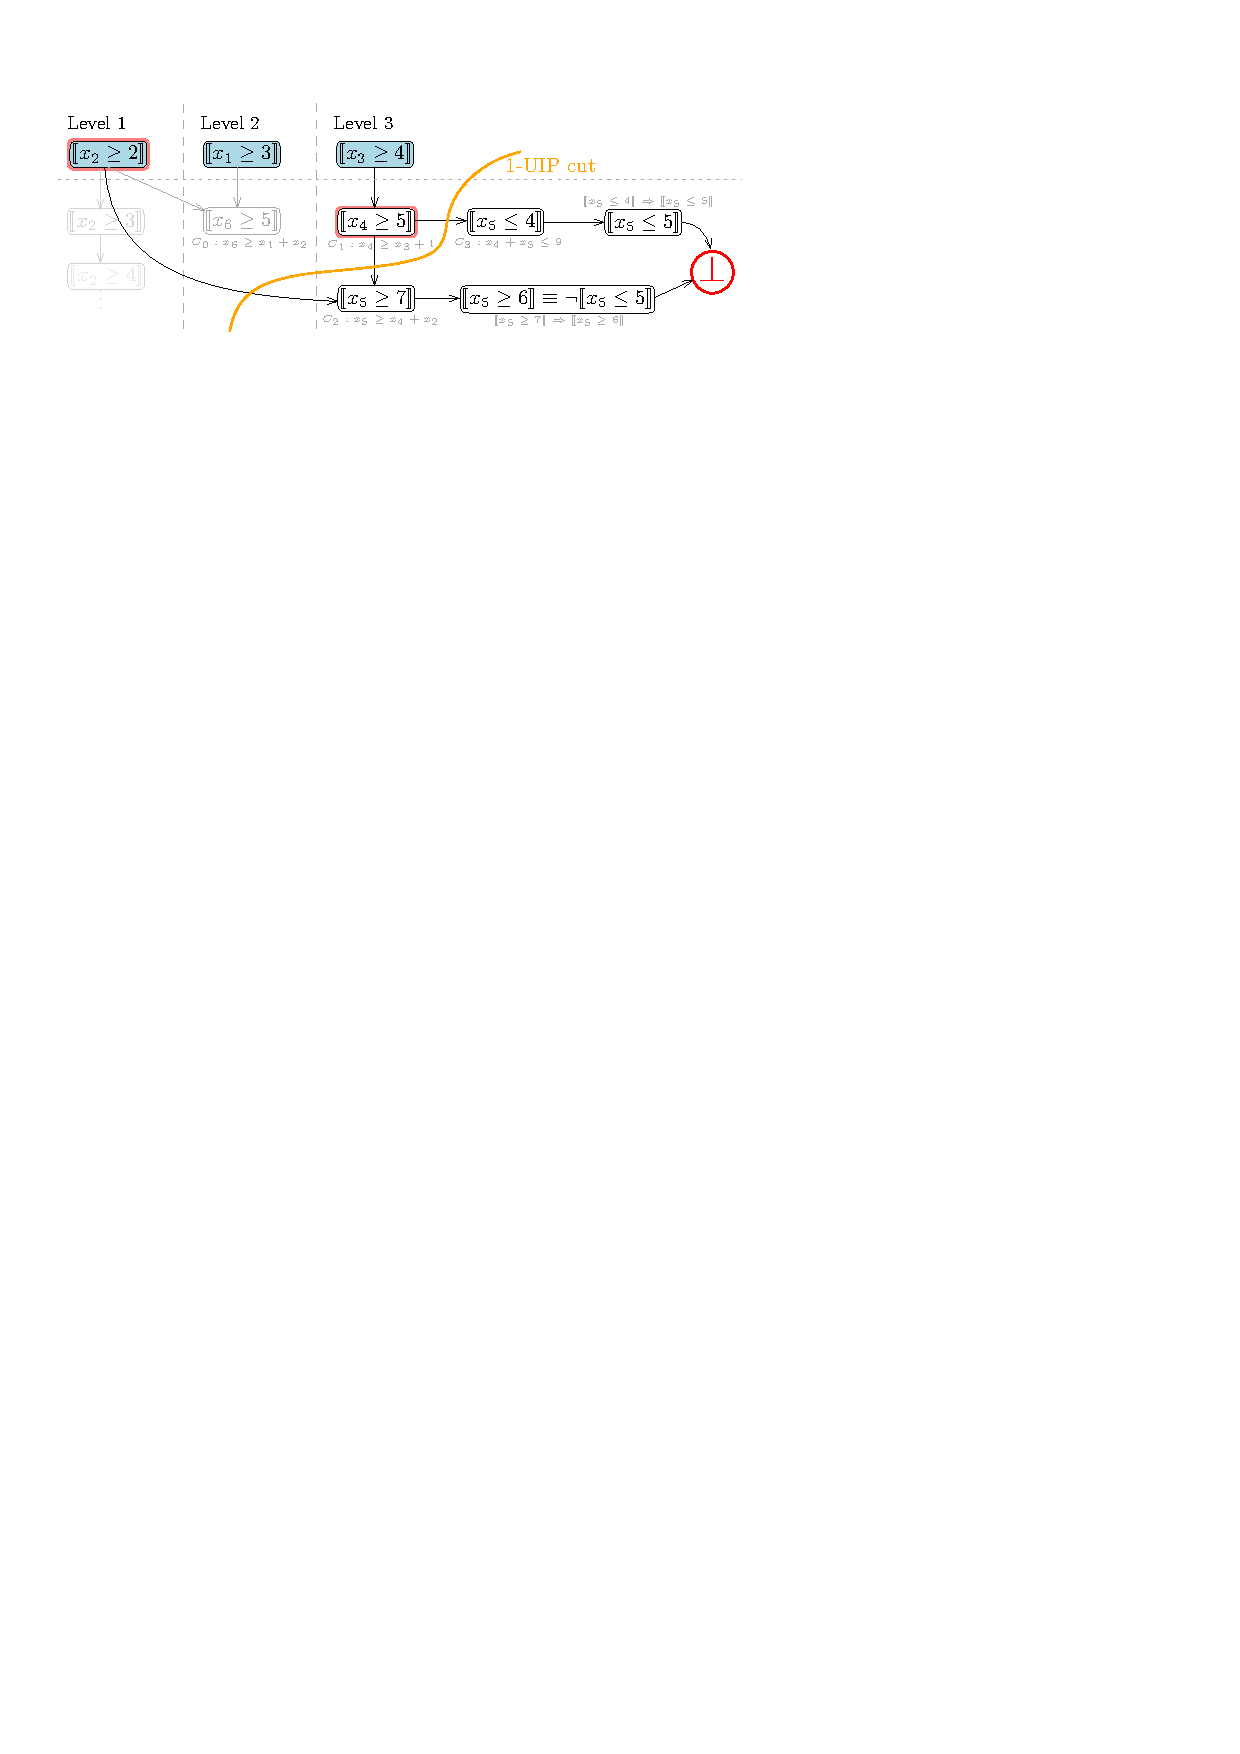
\includegraphics[width=\linewidth]{figures/conflict_analysis.pdf}
\caption{Implication graph for the trace: nodes are bound literals
$\bl{\cdot}$, blue for decisions and $\bot$ for the conflict, with the rule that
forced each propagated bound beneath it. The orange \emph{1-UIP cut} isolates the
dominator $x_4 \ge 5$ and the lower-level decision $x_2 \ge 2$ (ringed), whose
negation $\{\lnot\bl{x_4 \ge 5},\ \lnot\bl{x_2 \ge 2}\}$ is the learned nogood;
the faded branch is the off-path $x_6 \ge 5$ that analysis never visits.}
\label{fig:uipgraph}
\end{figure}

\textbf{The resolution.} Before the walk, one convention is worth stating. Each
bound on the trail holds as a \emph{true} fact, such as the $x_4 \ge 5$ the solver
set, whereas the clauses it appears in, both the failing clause and the reasons,
carry the corresponding \emph{negated} bound literal. Resolving on $x_4 \ge 5$
therefore means cancelling $\lnot\bl{x_4 \ge 5}$ in the working
clause against $\bl{x_4 \ge 5}$ in its reason. The
$\textsc{Reason}(\ell)$ the loop calls is a dispatch, not a lookup in some shared
table: when a propagator enqueues a bound it stamps that trail entry with its own
identifier, so the trail records which propagator set each $\ell$. Asking for
$\textsc{Reason}(\ell)$ calls exactly that propagator back to explain its
deduction, building the justifying clause on demand and caching it
(\srcla{sat\_base.h}{951}{Trail::Reason}, which indexes \code{propagators\_}
by the stored setter and invokes its \code{Reason}); decisions and unit facts
carry an empty reason and end the walk. This is the lazy clause generation of
\cref{sec:learning} at work: the reason exists only once conflict analysis
asks the propagator that produced $\ell$ for it. With this
convention in place, the algorithm keeps a working clause, initially the failing
clause, and repeatedly replaces the most recently assigned current-level bound by
its reason until exactly \textbf{one} current-level bound remains. It processes
bounds by decreasing trail index, which peels the conflict backward toward the
dominator. Formally, this is a short resolution loop:

\begin{algorithm}[htbp]
\caption{First-UIP conflict analysis (\code{ComputeFirstUIPConflict})}
\label{alg:uip}
\begin{algorithmic}[1]
\State $C \gets$ failing clause \Comment{the violated constraint}
\While{$C$ has more than one literal assigned at the current decision level}
  \State $\ell \gets$ the current-level literal of $C$ with the highest trail index
  \State $C \gets \big(C \setminus \{\ell\}\big) \,\cup\, \big(\textsc{Reason}(\ell) \setminus \{\lnot\ell\}\big)$ \Comment{reason = ask the propagator that set $\ell$}
\EndWhile
\State $u \gets$ the unique current-level literal remaining in $C$ \Comment{the 1-UIP}
\State \Return $C$ \Comment{learned nogood; backjump to \textnormal{\textsc{AssertionLevel}}$(C)$}
\end{algorithmic}
\end{algorithm}

Walking that loop on our trail makes the mechanics concrete:

\begin{itemize}
  \item \textbf{Start.} The working clause is the failing clause, the order-encoding
  consistency clause $\{\lnot\bl{x_5 \ge 7},\ \lnot\bl{x_5
  \le 5}\}$: the monotone link $\bl{x_5 \ge 7}
  \Rightarrow \bl{x_5 \ge 6}$, written with $\lnot\bl{x_5
  \le 5}$ in place of the bound literal $\bl{x_5 \ge 6}$ it
  equals. Both bounds were assigned at the current level, level 3, so the loop
  continues.
  \item \textbf{Resolve on $x_5 \ge 7$} (highest trail index, position 5). Its
  reason is $C_2$ acting on $x_4 \ge 5$ and $x_2 \ge 2$, giving the clause
  $\{\lnot\bl{x_4 \ge 5},\ \lnot\bl{x_2 \ge 2},\
  \bl{x_5 \ge 7}\}$, which says that $x_4 \ge 5$ and $x_2 \ge 2$
  together force $x_5 \ge 7$. Replacing $\lnot\bl{x_5 \ge 7}$ by
  the rest of that reason (writing $\odot$ for resolution) gives
  \[
    \begin{aligned}
    \{\lnot\bl{x_5 \ge 7},\ \lnot\bl{x_5 \le 5}\}
    &\odot
    \{\lnot\bl{x_4 \ge 5},\ \lnot\bl{x_2 \ge 2},\
      \bl{x_5 \ge 7}\} \\
    &= \{\lnot\bl{x_5 \le 5},\ \lnot\bl{x_4 \ge 5},\ \lnot\bl{x_2 \ge 2}\}.
    \end{aligned}
  \]
  Two current-level bounds remain, $x_5 \le 5$ and $x_4 \ge 5$, so the loop
  continues.
  \item \textbf{Resolve on $x_5 \le 5$} (position 4). This is the order-encoding
  step: $x_5 \le 5$ was forced not by a constraint but by the monotone link
  $x_5 \le 4 \Rightarrow x_5 \le 5$, whose clause is $\{\lnot\bl{x_5 \le 4},\ \bl{x_5 \le 5}\}$. Replacing $\lnot\bl{x_5
  \le 5}$ gives
  \[
    \begin{aligned}
    \{\lnot\bl{x_5 \le 5},\ \lnot\bl{x_4 \ge 5},\
      \lnot\bl{x_2 \ge 2}\}
    &\odot
    \{\lnot\bl{x_5 \le 4},\ \bl{x_5 \le 5}\} \\
    &= \{\lnot\bl{x_5 \le 4},\ \lnot\bl{x_4 \ge 5},\ \lnot\bl{x_2 \ge 2}\}.
    \end{aligned}
  \]
  The bounds $x_5 \le 4$ and $x_4 \ge 5$ are both current-level, so the loop
  continues.
  \item \textbf{Resolve on $x_5 \le 4$} (position 3). Its reason is $C_3$ acting on
  $x_4 \ge 5$, giving the clause $\{\lnot\bl{x_4 \ge 5},\
  \bl{x_5 \le 4}\}$, which says that $x_4 \ge 5$ forces
  $x_5 \le 4$. Replacing $\lnot\bl{x_5 \le 4}$ gives
  \[
    \{\lnot\bl{x_5 \le 4},\ \lnot\bl{x_4 \ge 5},\
      \lnot\bl{x_2 \ge 2}\}
    \odot
    \{\lnot\bl{x_4 \ge 5},\ \bl{x_5 \le 4}\}
    = \{\lnot\bl{x_4 \ge 5},\ \lnot\bl{x_2 \ge 2}\}.
  \]
  Only $x_4 \ge 5$ is now a current-level bound, since the other, $x_2 \ge 2$,
  belongs to level 1. Exactly \textbf{one} current-level bound remains, so the
  loop stops.
\end{itemize}

\textbf{The UIP.} The single remaining current-level bound is the
\textbf{first Unique Implication Point}, $x_4 \ge 5$. It is the one node at level
3 through which every conflict path runs, since both $x_5 \ge 7$ and $x_5 \le 5$
were forced by it. Negating it and moving it to the front gives the learned
clause
\[
  \textbf{Learned nogood: }
  \{\lnot\bl{x_4 \ge 5},\ \lnot\bl{x_2 \ge 2}\},
\]
which reads ``never have $x_4 \ge 5$ and $x_2 \ge 2$ at once,'' or equivalently
that whenever $x_2 \ge 2$ holds the bound $x_4 \le 4$ must follow. This is a fact
stated purely in bounds, sound everywhere in the tree rather than only on this
branch.

\textbf{Backjump.} The solver computes the \textbf{assertion level}: the highest
decision level among the learned clause's literals \emph{other than} the UIP
(\srcla{sat\_solver.cc}{1896}{ComputePropagationLevel}). Here that is the
level of $x_2 \ge 2$, namely level~1, so the solver retreats from level 3 straight
to level 1. Everything above level 1 is undone in the process: the level-2
decision $x_1 \ge 3$ and its propagation $x_6 \ge 5$ are popped along with the
level-3 cascade. Nothing in between is selectively kept; the undo is a plain
truncation of both trails to the end of level 1, leaving only level 1 and below.
The force of the \textbf{non-chronological backjump} is not that $x_1 \ge 3$
survives but that the solver does not stop at level 2 to retry it: that decision
had no part in the failure, so search resumes at level 1 instead.
One-level-at-a-time CP backtracking cannot make that jump.

\textbf{Assertion.} Back at level 1, $x_2 \ge 2$ is still true. So in the learned
clause $\{\lnot\bl{x_4 \ge 5},\ \lnot\bl{x_2 \ge 2}\}$ the literal $\lnot\bl{x_2 \ge 2}$ is false and
$\lnot\bl{x_4 \ge 5}$ is the only unassigned literal. The clause
is now \textbf{unit} and immediately propagates it, forcing $x_4 \le 4$
(\srcla{sat\_solver.cc}{486}{AddLearnedClauseAndEnqueueUnitPropagation}).
Search resumes already knowing a fact that cost one conflict to learn, and that
fact will fire automatically in every future branch where $x_2 \ge 2$ holds.

\textbf{Two finishing touches CP-SAT applies in practice:}

\begin{itemize}
  \item \textbf{Minimization.} Before storing the clause, CP-SAT applies
  self-subsuming resolution (\srcla{sat\_solver.cc}{2627}{MinimizeConflict}): any literal whose own reason is already implied
  by the other clause literals can be dropped, yielding a shorter, stronger
  nogood.
  \item \textbf{LBD scoring.} The clause's LBD is recorded
  (\srcla{sat\_solver.cc}{1926}{ComputeLbd}). Here the learned clause
  touches two distinct decision levels, so its LBD is 2. A low LBD marks it as a
  high-quality clause: it is more likely to be protected from clause-database
  cleanup, and it later feeds the restart heuristic (\cref{sec:restarts}).
\end{itemize}

That one trace exercises every part of the engine: propagators deduce with
reasons, the conflict resolves those reasons to a unique dominator, the
dominator becomes a permanent learned clause, and a non-chronological backjump
turns the lesson into immediate forward progress.

% Source (VERIFIED): "Search stats" table column "Conflicts" = FormatCounter(r.num_conflicts())
%   in ortools/sat/stat_tables.cc:91. The response field "conflicts:"
%   (cp_model_solver.cc:712) is NOT a portfolio sum -- it is one worker's
%   num_failures(), copied by the statistics postprocessor (see the portfolio box in
%   the parallelization section); a real 24-worker log showed conflicts:0 in the
%   summary while the 'core' row recorded ~920k.
% Empirical (real CP-SAT logs): Conflicts <= Branches in EVERY worker observed
%   (a conflict is resolved by a backjump that undoes >=1 decision). The diagnostic
%   is the ratio: Conflicts ~ Branches => learning from almost every decision;
%   Conflicts << Branches (or 0) => mostly feasible descent.
\begin{platypuslog}[htb]
Each conflict resolution increments the \code{Conflicts} column of the per-worker
\textsf{Search stats} table: one learned nogood per conflict. In ordinary search,
a conflict is resolved by a backjump that undoes at least one decision, so
\code{Conflicts} stays at or below \code{Branches} in each worker. The useful
diagnostic is how close the two counts are. A \code{Conflicts} count that is a
large fraction of \code{Branches} indicates a worker learning from nearly every
decision; \code{Conflicts} tiny compared with \code{Branches}, or zero, indicates
a worker mostly descending feasibly without hitting dead ends.
\end{platypuslog}
